\documentclass[11pt,a4paper]{article}

\usepackage{iftex}
\ifPDFTeX
  \usepackage[T1]{fontenc}
  \usepackage[utf8]{inputenc}
  \usepackage{lmodern}
\else
  \usepackage{fontspec}
\fi
\usepackage[margin=2.3cm]{geometry}
\usepackage{amsmath,amssymb}
\usepackage{booktabs}
\usepackage{tabularx}
\usepackage{graphicx}
\usepackage{float}
\usepackage{enumitem}
\usepackage{xcolor}
\usepackage{tikz}
\usetikzlibrary{positioning,arrows.meta}
\usepackage[colorlinks=true,linkcolor=blue!50!black,urlcolor=blue!50!black]{hyperref}

\newcolumntype{Y}{>{\raggedright\arraybackslash}X}
\newcommand{\code}[1]{\texttt{\detokenize{#1}}}
\newcommand{\RMSE}{\operatorname{RMSE}}

\title{How We Calibrated WOFOST to Texcoco Farm Yields\\[0.3em]\large What was done, why, and how to read the results}
\author{Gradient Descent Farmers --- companion to the technical report}
\date{\today}

\begin{document}
\maketitle

\section*{1. In one paragraph}

Before calibration, the crop simulator predicted yields 2.5 to 5 times higher than what Texcoco farmers report to the
Mexican government (6.5 vs 2.6 t/ha for maize, 6.1 vs 1.8 for barley, 9.8 vs 1.9 for faba bean). We picked a few
model settings (``knobs'') with a clear physical meaning and tried many combinations. For each crop we kept the
combination whose simulated yields came closest to the observed yields of 2006--2021, and we checked it on 2022--2025.
After calibration the simulated averages are within 0.06--0.25 t/ha of the observed ones in the fit years. But the
calibrated model does \textbf{not} predict individual years better than simply using the observed 2006--2021
average, and for maize it does worse. Calibrated yields are realistic \emph{levels} for scenarios; they are not
forecasts. A second finding matters for the rotation work: once calibrated, maize no longer yields more after barley
or faba bean than after maize.

This is the second version of the calibration. An independent review of the first version found that it compared
maize with the wrong mix of rotations and contradicted a local fertilizer trial; Section~7.2 explains what changed.

\section*{2. What ``calibration'' means here}

WOFOST, the crop model we use, does not learn from yields. It computes a yield day by day from weather, soil and
about a hundred crop parameters (see the companion \emph{What Kind of Model Is WOFOST?}). Those parameters come from
field experiments in Europe: they describe modern varieties grown with good weed, pest and fertilizer management.
Texcoco's rainfed farms are different, so the model's yields are attainable yields, not farm yields.

\textbf{Calibration} means adjusting a small number of those parameters so that the model's output matches observed
data for the place we care about. It is a curve fit, but of a few physically meaningful numbers inside the model,
not of the yield itself.

\paragraph{Why not just multiply the yields by a correction factor?}
The farmer notebook did exactly that: it multiplied every maize yield by about 0.4, barley by 0.28 and faba bean by 0.18.
That fixes the average but nothing else:
\begin{itemize}[nosep]
  \item the model still believes fertilizer, frost and drought act on a 6--10 t/ha crop, so the size of every
        scenario effect (``20\% less rain'', ``no fertilizer'') is wrong;
  \item the same factor is applied in every year, whatever happened in that year.
\end{itemize}
Changing parameters \emph{inside} the model lets the lower yield interact with water, nitrogen and frost the way a
real low-input crop would.

\section*{3. The ingredients}

\subsection*{3.1 Observed yields: SIAP}

SIAP (Servicio de Información Agroalimentaria y Pesquera) publishes, every year and for every municipality, the area
sown, the area harvested, the area lost and the production of each crop. We keep the rows for Texcoco (state 15,
municipality 99), the spring--summer cycle and rainfed land (\code{farm_tool.siap_texcoco}). From them we use the
\textbf{yield per sown hectare}:
\begin{equation}
  y^{\mathrm{obs}} = \frac{\text{production (t)}}{\text{sown area (ha)}}.
\end{equation}
Dividing by the \emph{sown} area (not the harvested area) counts fields that were lost to frost or drought as zero
yield. That is what a failed season looks like in the model, so the two are comparable. In 2011 and 2019, for
example, 51\% and 64\% of the maize area was lost, and the yield per sown hectare falls to 1.0 and 0.8 t/ha.

\begin{table}[H]
\centering\small
\begin{tabular}{llccc}
\toprule
Crop & Years with data & Mean 2006--2021 & Mean 2022--2025 & Sown area, 2022--2025 \\
\midrule
Maize & 2005--2025 & 2.56 (16 years) & 2.98 & 900--1,400 ha \\
Barley & 2008--2025 & 1.78 (14 years) & 1.55 & 4--9 ha \\
Faba bean & 2005--2019, 2022--2025 & 1.94 (14 years) & 1.17 & 10--12 ha \\
\bottomrule
\end{tabular}
\caption{The observations used (yields in t/ha per sown hectare). Barley has no data before 2008 and faba bean none
for 2020--2021.}
\end{table}

\subsection*{3.2 Simulated yields, combined as SIAP would see them}

The simulator (\code{wofost_rotations.py}) runs four rotations (maize every year; maize--barley; maize--faba bean;
maize--barley--faba bean) from 2005 to 2025. Every \emph{phase} of a rotation is simulated: maize--barley is run once
starting with maize and once starting with barley, so every crop appears every year. Seasons are chained, so the
water and nitrogen left by one crop start the next one. The yield we compare is the \textbf{water- and
nitrogen-limited yield} (rainfed, with fertilizer, with the grain-N constraint), the most realistic of the three
production levels the simulator computes. The first year, 2005, is a ``spin-up'' that starts from assumed soil water
and nitrogen, so it is left out.

SIAP reports one number per crop and year for the whole municipality, so the simulated seasons must be combined into
one number in the same way. For maize, the share of fields following each crop matters a lot, and SIAP tells us
roughly what it is. Maize after barley can cover at most the barley area of the year before, and the same holds for
faba bean:
\begin{equation}
  w^{\text{barley}}_t = \frac{\text{barley area}_{t-1}}{\text{maize area}_t},\qquad
  w^{\text{faba}}_t = \frac{\text{faba bean area}_{t-1}}{\text{maize area}_t},\qquad
  w^{\text{maize}}_t = 1 - w^{\text{barley}}_t - w^{\text{faba}}_t,
\end{equation}
and the simulated maize yield of year \(t\) is the weighted average of maize after each crop:
\begin{equation}
  y^{\mathrm{sim}}_{\text{maize},t} = \sum_{p\,\in\,\{\text{maize, barley, faba}\}} w^{p}_t\;
  \bar Y_{\text{maize after }p,\ t}.
\end{equation}
Over 2006--2021 barley and faba bean areas are only 7.4\% of the next year's maize area on average (at most 24.8\% in
2009, and under 3\% since 2019; 2023's maize, for example, had 21~ha of 2022 barley and faba bean against 1,390~ha). So almost all Texcoco maize follows maize. The rest
of the area is assumed to follow maize too: SIAP has no field histories, and other preceding crops (oats, for
example) are not simulated. Barley and faba bean are averaged over all rotations and phases, since SIAP cannot tell
what they follow. This is \code{farm_tool.simulated_like_siap}, used by the calibration and by \code{farm_gap} in the
notebook.

\paragraph{Why this matters.} The first version of the calibration averaged maize over the four rotations equally,
as if three quarters of the fields followed barley or faba bean. Re-weighted by the real areas, its calibrated maize
fell from 2.35 to 1.97 t/ha in the fit years and to 1.90 in 2022--2025 (holdout RMSE 2.27 instead of 0.89). Its good
holdout score depended on the wrong weighting.

\subsection*{3.3 Fit years and holdout years}

A model with enough knobs can match any short series, including its noise, and then fail on new years. This is
called \emph{overfitting}. To check for it, the years are split:
\begin{itemize}[nosep]
  \item \textbf{Calibration (fit) years, 2006--2021}: the only years the search looks at when choosing knob values.
  \item \textbf{Holdout years, 2022--2025}: never used to choose knob values. Four years is little, so the holdout
        tells us about the level more than about year-to-year agreement.
\end{itemize}
The holdout is not pristine, though: while designing the first version we looked closely at 2023 (Section~5) and at
diagnostics that printed holdout scores. The diagnostics now score fit years only.

\section*{4. How a fit is scored, and what it is compared with}

For one crop and the \(n\) years with an observation, let \(e_t = y^{\mathrm{sim}}_t - y^{\mathrm{obs}}_t\) be
the error in year \(t\). We report:
\begin{align}
  \text{Level:}\quad & \bar y^{\mathrm{sim}} \text{ vs } \bar y^{\mathrm{obs}}
      \quad\text{(the two means; their ratio is the old correction factor)}\\
  \text{Bias:}\quad & \bar e = \frac{1}{n}\sum_t e_t \quad\text{(positive = model too high)}\\
  \text{RMSE:}\quad & \RMSE = \sqrt{\frac{1}{n}\sum_t e_t^2} \quad\text{(typical size of the error, in t/ha)}\\
  \text{Correlation:}\quad & r = \frac{\sum_t (y^{\mathrm{sim}}_t - \bar y^{\mathrm{sim}})(y^{\mathrm{obs}}_t - \bar y^{\mathrm{obs}})}
      {\sqrt{\sum_t (y^{\mathrm{sim}}_t - \bar y^{\mathrm{sim}})^2}\sqrt{\sum_t (y^{\mathrm{obs}}_t - \bar y^{\mathrm{obs}})^2}}
\end{align}
\(r\) runs from \(-1\) to 1. It measures whether good and bad years line up (1 = perfectly, 0 = no relation),
whatever the level. With 16 years, \(r\) must be above about 0.5 to be distinguishable from zero.

\paragraph{The search minimizes RMSE.} It is useful to know that
\begin{equation}
  \RMSE^2 = \bar e^{\,2} + \operatorname{SD}(e)^2,
\end{equation}
so RMSE punishes both a wrong level (\(\bar e\)) and wrong year-to-year swings (\(\operatorname{SD}(e)\)). When the
model's swings do not line up with the observed ones, the cheapest way to lower RMSE is to make the model swing
\emph{less}, or to settle slightly below the observed level if higher yields come with bigger swings.

\paragraph{Naive baselines.} A model is only useful if it beats a trivial prediction. We compare every result with
two of them, both computed from SIAP alone:
\begin{itemize}[nosep]
  \item \textbf{Climatology}: every year gets the 2006--2021 SIAP average of that crop.
  \item \textbf{Persistence}: every year gets last year's SIAP yield (years whose previous year has no observation are
        left out).
\end{itemize}
The \textbf{skill score} \(1 - \RMSE/\RMSE_{\text{climatology}}\) is positive when the model beats climatology,
zero when it ties and negative when it does worse.

\section*{5. Diagnosis: why is the default model so far off?}

Before fitting anything, we changed one assumption at a time and reran all rotations
(\code{python -m src.crop_models.calibration --sensitivity}). Table~\ref{tab:sens} summarizes the results.

\begin{table}[H]
\centering\small
\begin{tabular}{lrrrrr}
\toprule
Change from the default & Maize & Barley & Faba bean & Maize \(r\) & Maize ended by frost \\
\midrule
None (default) & 6.47 & 6.15 & 9.79 & 0.35 & 69\% \\
Phenology \(\times 0.8\) (shorter cycle) & 9.41 & 5.56 & 9.80 & 0.39 & 25\% \\
Phenology \(\times 0.65\) & 10.64 & 4.24 & 8.22 & 0.40 & 6\% \\
Photosynthesis \(\times 0.5\) & 3.41 & 2.77 & 2.53 & \(-0.02\) & 69\% \\
Fertilizer N recovery 0.25 (not 0.5) & 4.16 & 4.97 & 9.77 & 0.39 & 69\% \\
Soil N mineralization halved & 4.60 & 3.83 & 9.74 & 0.38 & 69\% \\
Frost kills at \(-2\,^\circ\)C (not \(0\,^\circ\)C) & 6.79 & 6.15 & 9.89 & 0.35 & 44\% \\
Soil 50 cm deep (not 100 cm) & 6.06 & 6.16 & 9.79 & 0.35 & 69\% \\
\midrule
SIAP (observed) & 2.56 & 1.78 & 1.94 & & \\
\bottomrule
\end{tabular}
\caption{One-at-a-time sensitivity: mean simulated yield 2006--2021 (t/ha) over the years with SIAP data, maize
weighted by SIAP areas. Saved by \code{--sensitivity} as \code{sensitivity.csv}.}
\label{tab:sens}
\end{table}

What the table and the model's internal variables tell us:

\begin{enumerate}[leftmargin=*]
  \item \textbf{The crop parameters describe high-yield European crops.} Without water or nitrogen limits
        (``potential'' yield) the default simulates 11.2 t/ha of maize, 12.0 of barley and 10.0 of faba bean.
        Rain barely matters on average: the 100 cm soil stores 236 mm of plant-available water and May--October
        brings about 770 mm on average, so the rainfed yields are the same as the potential ones.
  \item \textbf{Nitrogen is the only brake in the default model, and only on maize and barley.} Default maize takes
        up about 150 kg of N/ha: 80 kg from fertilizer (160 kg/ha applied, of which the model lets the crop recover
        half) and about 64 kg per season from the soil's own organic matter (mineralization). Halving either source
        lowers maize by about 2 t/ha. Faba bean is a legume that takes 80\% of its nitrogen from the air, so nothing
        reduces it.
  \item \textbf{Phenology and frost.} NASA POWER weather comes from a grid cell whose average elevation is
        2,633 m, about 380 m above the fields at El Batán. Air cools about 6.5\,\(^\circ\)C per km of altitude, so
        the weather the model sees is roughly 2.5\,\(^\circ\)C colder than the fields. Maize development is driven by
        accumulated temperature, so it is slow. The default maize flowers about 87 days after sowing (plausible for
        Valles Altos hybrids) but then needs about 100 more days to fill its grain. In 69\% of seasons the first
        frost (a night at or below 0\,\(^\circ\)C) ends the crop before it matures; when it matures, the median
        date is December 5.
  \item \textbf{Frost threshold and soil depth matter little.} Neither changes the mean by more than 0.4 t/ha. (The
        ``frost kills at \(-2\,^\circ\)C'' row means \emph{fewer} frosts; the \code{frost_minus2} scenario of the
        technical report means colder nights, i.e.\ \emph{more} frosts.)
  \item \textbf{Photosynthesis is a strong level lever but erases the year pattern.} Halving it brings all three crops
        much closer to SIAP, but maize's correlation drops from 0.35 to about 0.
\end{enumerate}

\paragraph{Why does continuous maize almost fail in 2023 in the default model?} SIAP reports 2023 as Texcoco's best
maize year (4.0 t/ha). In the default model, maize after barley or faba bean does well in 2023 (11--13 t/ha), but
maize after maize nearly fails (0.01 t/ha):
\begin{enumerate}[nosep]
  \item the 2022 maize was sown late (June 15) and kept transpiring until January 5, 2023;
  \item on March 1, 2023 the soil therefore held under 10 mm of water the plant could use, against 130--200 mm when
        barley or faba bean had been grown in 2022 (no rain falls in the dry season to refill it);
  \item the 2023 crop was sown on May 15, after about 24 mm of early-May rain, and then June was almost rainless
        (a 28-day dry spell; 2023 had the driest May--October of 2005--2025 in the POWER data, 478 mm);
  \item with no water to take up, the seedlings could not grow; their leaf area shrank from 0.05 to 0.003 and never
        recovered. WOFOST has no ``re-sowing'', which a farmer would do.
\end{enumerate}
Because almost all Texcoco maize follows maize (Section~3.2), this failure dominated the default model's 2023. The
calibrated model's shorter maize cycle (chosen on 2006--2021 only) avoids it: calibrated continuous maize gives
2.0 t/ha in 2023.

\section*{6. The knobs, and the fertilizer-trial constraint}

We use four knobs, each tied to a mechanism found in Section~5. The defaults reproduce the uncalibrated model
exactly.

\begin{table}[H]
\centering\small
\begin{tabularx}{\linewidth}{lllY}
\toprule
Knob & WOFOST parameters changed & Default & What it represents \\
\midrule
Phenology scale \(s\) & TSUM1, TSUM2 \(\times s\) & 1 & A shorter or longer-cycle variety \\
Photosynthesis scale \(p\) & AMAX\_REF, AMAX\_SLP, EFFTB \(\times p\) & 1 & Losses WOFOST does not simulate: weeds,
  pests, diseases, uneven plant stands, landrace genetics \\
Fertilizer N recovery \(f\) & share of each N dose the crop can access & 0.5 & Lower doses than the 160 kg/ha plan,
  losses to leaching and volatilization \\
Soil mineralization \(m\) & N released per season \(= m \times\) soil total N & 0.5\% & Fertility of the soil organic
  matter (one value for the site) \\
\bottomrule
\end{tabularx}
\caption{The calibration knobs. The first three are set per crop; mineralization is shared by all crops.}
\end{table}

\paragraph{Phenology (TSUM).} WOFOST tracks a development stage \(D\) that goes from 0 at emergence to 1 at
flowering and 2 at maturity. Each day it grows by the day's effective temperature divided by a thermal-time
requirement:
\begin{equation}
  D_{t+1} = D_t + \frac{T_{\mathrm{eff}}(t)}{\mathrm{TSUM1}}\ (D<1), \qquad
  D_{t+1} = D_t + \frac{T_{\mathrm{eff}}(t)}{\mathrm{TSUM2}}\ (D\ge 1),
\end{equation}
where, for maize, \(T_{\mathrm{eff}} = \min(\max(T - 6, 0), 24)\) in \(^\circ\)C\,day. Multiplying TSUM1 and TSUM2
by \(s<1\) makes every stage arrive sooner. Table~\ref{tab:phen} shows what this means in days after sowing at
Texcoco. Phenology depends only on the sowing date and temperature, so it is the same in every rotation.

\begin{table}[H]
\centering\small
\begin{tabular}{llrrr}
\toprule
Crop & Phenology scale & Days to flowering & Days to end of season & Seasons reaching maturity \\
\midrule
Maize & 1.0 (default) & 87 & 191 & 31\% \\
      & 0.8 (calibrated) & 72 & 155 & 75\% \\
Barley & 1.0 (default) & 63 & 117 & 88\% \\
       & 0.9 (calibrated) & 57 & 107 & 100\% \\
Faba bean & 1.0 (default) & 57 & 145 & 75\% \\
          & 0.9 (calibrated) & 52 & 130 & 88\% \\
\bottomrule
\end{tabular}
\caption{Simulated phenology, medians over the 16 seasons of 2006--2021 (median sowing: maize May 27, barley July 1,
faba bean June 16). A season ends at maturity, at the first frost, or on February 28.}
\label{tab:phen}
\end{table}

\paragraph{Photosynthesis.} In WOFOST 8.1 the maximum CO\(_2\) uptake of a leaf depends on its nitrogen content:
\(A_{\max} = \text{CO2 factor} \times \text{temperature factor} \times \min(\mathrm{AMAX\_REF},\
\mathrm{AMAX\_SLP}\cdot \mathrm{SLN})\), and EFF is the light-use efficiency of a leaf in dim light. Scaling all
three by \(p\) scales each leaf's CO\(_2\) uptake, and so the crop's daily sugar production, by \(p\). (The scaling is
exact while the scaled \(A_{\max}\) stays above 2~kg/ha/h. PCSE's light-response curve divides by
\(\max(2, A_{\max})\), so for leaves with very little nitrogen the reduction is slightly stronger: 0.456 instead of
0.47 in one check.) Maintenance respiration is not scaled, so yield falls faster than \(p\); extrapolating the grid, maize
yield would reach zero near \(p \approx 0.3\). Everything downstream (leaf growth, roots, grain, N demand) responds to it, which is why
this works better than multiplying the final yield.

\paragraph{Nitrogen.} Each fertilizer dose of \(F\) kg N/ha makes \(f \cdot F\) available to the crop; the rest is
lost. The soil also releases \(m \times 12{,}709\) kg N/ha (IGBP total N in 0--100 cm) per season, spread evenly over
the first 150 days from March 1. With the defaults that is \(0.005 \times 12{,}709 \approx 64\) kg. The simulator caps
this release at 100 kg N/ha per season, the valid range of the PCSE parameter it feeds (\code{NSOILBASE}); any
\(m\) above 0.79\% gives 100 kg.

\paragraph{The fertilizer-trial constraint.} SIAP tells us how much a field yields, not where its nitrogen came from.
The first version of the calibration lowered maize yields by cutting nitrogen (fertilizer recovery 0.2 and half the
mineralization). Its unfertilized maize then fell to 0.29 t/ha against 2.35 fertilized, a ratio of 0.12. The only
local nitrogen data in the repository say the opposite: in a rainfed hybrid trial at INIFAP's Texcoco station,
maize gave 5.2 t/ha without fertilizer and 5.6 t/ha with 160 kg N/ha, a ratio of 0.93 (Alonso-Sánchez et al.\ 2023,
\href{https://doi.org/10.28940/terra.v41i0.1577}{doi:10.28940/terra.v41i0.1577}). So maize candidates are now also
run without fertilizer, and only those whose continuous-maize ratio
\begin{equation}
  \rho = \frac{\text{mean yield without fertilizer, 2006--2021}}{\text{mean yield with fertilizer, 2006--2021}}
\end{equation}
is within 0.1 of 0.93 are eligible (\code{within_trial}). The trial is one research-station experiment, so applying it
to the whole municipality is an assumption; the tolerance of 0.1 reflects that.

\paragraph{Can the model reproduce the trial itself?} The constraint uses only the trial's \emph{ratio}. To check the
absolute yields, we ran continuous maize with and without fertilizer at station-like settings
(\code{python -m src.crop_models.calibration --station-check}):
\begin{center}\small
\begin{tabular}{rrrrrr}
\toprule
Phenology & Photosynthesis & Soil N (kg/ha per season) & Unfertilized & Fertilized & Ratio \\
\midrule
\multicolumn{3}{l}{\textbf{Texcoco trial}} & \textbf{5.2} & \textbf{5.6} & \textbf{0.93} \\
\(\times 1\) & \(\times 1\) & 64 (default) & 1.92 & 6.48 & 0.30 \\
\(\times 1\) & \(\times 1\) & 100 (cap) & 3.96 & 8.37 & 0.47 \\
\(\times 0.8\) & \(\times 1\) & 100 (cap) & 5.81 & 11.86 & 0.49 \\
\(\times 0.8\) & \(\times 0.65\) & 100 (cap) & 5.55 & 6.32 & 0.88 \\
\(\times 0.8\) & \(\times 0.6\) & 95 & 4.65 & 5.01 & 0.93 \\
\(\times 0.8\) & \(\times 0.6\) & 64 (default) & 3.99 & 5.01 & 0.80 \\
\bottomrule
\end{tabular}
\end{center}
Mean yields 2006--2021 (t/ha), fertilizer recovery 0.5. Three things follow:
\begin{itemize}[nosep]
  \item \textbf{At full photosynthesis no setting matches.} 5.2 t/ha without fertilizer is reachable only with the
        shorter cycle and the most soil N the simulator allows, and then fertilized maize gives 11.9 t/ha, twice the
        trial. Even station-managed maize sits well below WOFOST's European parameters.
  \item \textbf{The trial is matched with photosynthesis \(\times 0.6\)--\(0.65\) and 95--100 kg of soil N per season.}
        With the default 64 kg, unfertilized maize never exceeds 4.3 t/ha. So the station soil supplies about 50\%
        more nitrogen than the model's default, and possibly more, since the match sits at the 100 kg cap.
  \item \textbf{The farm-level constraint is weaker than it looks.} At the farm level (about 2.3 t/ha), calibrated maize
        takes up only about 60--68 kg of N per season, about what the default soil releases on its own (64 kg). Every
        candidate with low photosynthesis therefore passes, and the band even accepts no fertilizer response at all
        (the chosen candidate has 0.995, against the trial's 0.93). What the constraint really rules out is explaining
        the farm gap with nitrogen alone at full photosynthesis (ratio about 0.26). It does not show how much nitrogen
        farm soils supply.
\end{itemize}

\paragraph{How the knobs reach the model.} The calibration is passed to \code{simulate_rotations(..., calibration=...)}
as a dictionary. Crop parameters are applied as PCSE \emph{overrides} on the parameter provider of each season.
(Editing the crop parameter dictionary directly does not work: PCSE reloads the variety's parameters when the
crop is sown.) When no calibration is passed, the code takes exactly the old path: a rerun of the default baseline,
\code{no_fertilizer} and \code{canicula50} reproduces the saved CSVs exactly.

\section*{7. The search}

\subsection*{7.1 Grid search, one crop at a time}

A \textbf{grid search} lists a few values for each knob and simulates every combination (a ``candidate''). For
each candidate we simulate the rotations that contain the crop, compute the crop's RMSE over 2006--2021, and keep
the eligible candidate with the lowest RMSE. Figure~\ref{fig:loop} shows the loop.

\begin{figure}[H]
\centering
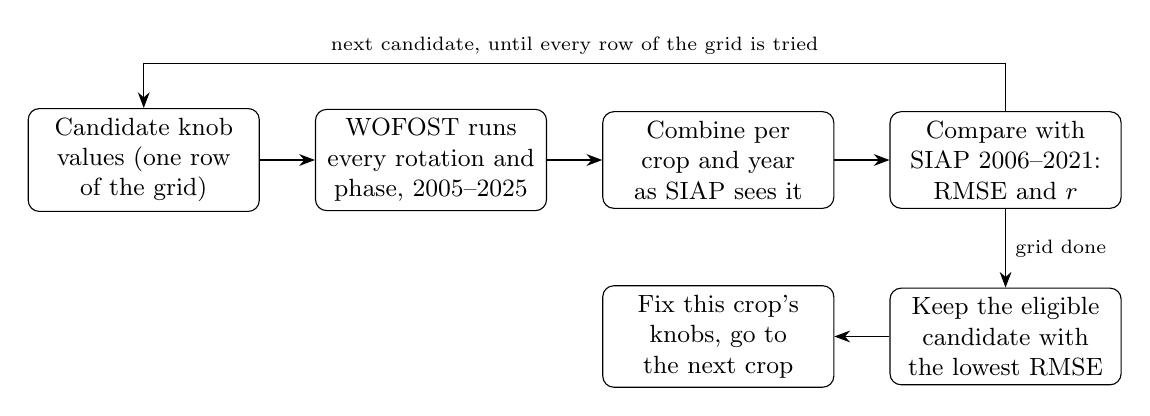
\begin{tikzpicture}[node distance=4mm and 7mm, box/.style={draw, rounded corners, align=center, font=\small,
  minimum height=12mm, text width=27mm}, >={Stealth[length=2mm]}]
\node[box] (cand) {Candidate knob values (one row of the grid)};
\node[box, right=of cand] (sim) {WOFOST runs every rotation and phase, 2005--2025};
\node[box, right=of sim] (avg) {Combine per crop and year as SIAP sees it};
\node[box, right=of avg] (cmp) {Compare with SIAP 2006--2021: RMSE and \(r\)};
\node[box, below=10mm of cmp] (best) {Keep the eligible candidate with the lowest RMSE};
\node[box, left=of best] (next) {Fix this crop's knobs, go to the next crop};
\draw[->] (cand) -- (sim); \draw[->] (sim) -- (avg); \draw[->] (avg) -- (cmp);
\draw[->] (cmp.north) -- ++(0,6mm) -| node[pos=0.25, above, font=\scriptsize]{next candidate, until every row of the grid is tried} (cand.north);
\draw[->] (cmp) -- node[right, font=\scriptsize]{grid done} (best);
\draw[->] (best) -- (next);
\end{tikzpicture}
\caption{The calibration loop. Maize candidates are also run without fertilizer to check the trial constraint. The
holdout years 2022--2025 never enter it.}
\label{fig:loop}
\end{figure}

Trying every combination of all knobs for all three crops at once would take days, so the crops are fitted one at
a time (``coordinate search''):
\begin{enumerate}[nosep]
  \item \textbf{Barley} (15 candidates): phenology \(\{0.8, 0.9, 1\}\), photosynthesis
        \(\{0.4, 0.425, 0.45, 0.475, 0.5\}\), N recovery 0.5. The fine photosynthesis steps matter: barley's level
        climbs about 0.3 t/ha per step.
  \item \textbf{Faba bean} (15): the same grid. Its N recovery barely matters because it fixes its own N.
  \item \textbf{Maize} (88), with barley and faba bean at their fitted values: phenology \(\{0.8, 1\}\), photosynthesis
        \(\{0.35, 0.4, 0.45, 0.46, 0.47, 0.48, 0.49, 0.5, 0.6, 0.75, 1\}\), and four nitrogen supplies (fertilizer
        recovery, mineralization): (0.2, 0.25\%), the first version's choice; (0.5, 0.5\%), the defaults;
        (0.5, 0.75\%); and (0.5, 1\%), which the 100 kg cap turns into 100 rather than 127 kg/season. Each maize
        candidate is also run without fertilizer.
\end{enumerate}
Maize goes last because it depends on its partners (it inherits the water and nitrogen they leave) more than they
depend on it. To save time, the search only simulates the water- and N-limited level. The search takes about
13 minutes on 8 processor cores; the maize photosynthesis values 0.46--0.49 were added in a second pass after the
first pass showed the level jumping from 2.0 to 2.8 t/ha between 0.45 and 0.5 (Figure~\ref{fig:maize}).
\code{fit_history.csv} holds every candidate of both passes.

\paragraph{Ties and grid edges.} RMSE and \(r\) are compared to three decimals; equal RMSE goes to the higher
correlation, and then to the candidate closest to the defaults, measured as \(\sum_k |v_k/\text{default}_k - 1|\). The
search also reports choices on the edge of the grid, since the best value may lie outside it.

\subsection*{7.2 How the calibration got here}

\begin{table}[H]
\centering\small
\begin{tabularx}{\linewidth}{lYY}
\toprule
Version & What the search chose & What we learned and changed \\
\midrule
1a & Maize phenology \(\times 0.6\), photosynthesis \(\times 0.6\), N recovery 0.25: all on the edge of the grid &
  \(\times 0.6\) means flowering 56 days after sowing, a variety not grown in Texcoco. Phenology was limited to
  \(\times 0.8\)--1. \\
1b--1d & Maize at default phenology and photosynthesis, with less and less N: recovery 0.15, then 0.05, then 0.2 with
  half the mineralization (mean 2.35, RMSE 0.71, \(r\) 0.39) & Published as the first calibration. \\
Review & An independent review found that (i) maize was averaged over rotations equally, though almost all Texcoco
  maize follows maize; (ii) the model did not beat the SIAP average; (iii) the N choice sat on the edge of the grid
  and contradicted the Texcoco fertilizer trial; (iv) barley's \(\times 0.8\) phenology was an artifact of a coarse
  grid & Maize is now weighted by SIAP areas; baselines are reported; maize candidates must keep the trial's fertilizer
  response, may lower photosynthesis, and can have more soil N; barley and faba bean get finer photosynthesis
  steps; diagnostics score fit years only. \\
2 (current) & Maize phenology \(\times 0.8\), photosynthesis \(\times 0.47\), default N supply; barley and faba bean
  phenology \(\times 0.9\), photosynthesis \(\times 0.475\) & See Section~8. \\
\bottomrule
\end{tabularx}
\caption{The versions of the calibration. A choice on the edge of the grid means the best value may lie outside it.}
\end{table}

Two limits are deliberate and come from agronomy, not from the fit:
\begin{itemize}[nosep]
  \item \textbf{Phenology at least \(\times 0.8\)}, to keep crop calendars realistic. Maize sits on this bound.
  \item \textbf{Photosynthesis at least about \(\times 0.35\)}. Below that the crops barely establish.
\end{itemize}
Maize's N supply is also reported as ``on the edge'', but that is a tie: once photosynthesis is low enough to match
the farm level, nitrogen no longer limits maize, so the default and higher N supplies give the same yields and the
tie goes to the defaults.

\section*{8. Results}

\begin{table}[H]
\centering\small
\begin{tabular}{lrrrl}
\toprule
Crop & Phenology & Photosynthesis & Fertilizer N recovery & \\
\midrule
Maize & \(\times 0.8\) & \(\times 0.47\) & 0.5 (default) & \\
Barley & \(\times 0.9\) & \(\times 0.475\) & 0.5 (default) & \\
Faba bean & \(\times 0.9\) & \(\times 0.475\) & 0.5 (default) & \\
Site & \multicolumn{4}{l}{Soil mineralization 0.5\% of total N per season (default, about 64 kg N/ha)} \\
\bottomrule
\end{tabular}
\caption{The fitted knobs, stored as \code{CALIBRATED} in \code{src/crop_models/calibration.py}. 56 of the 88 maize
candidates passed the trial constraint; the chosen one has a fertilizer ratio of 0.995.}
\end{table}

\begin{table}[H]
\centering\footnotesize
\setlength{\tabcolsep}{4pt}
\begin{tabular}{llrrrrrrr}
\toprule
 & & \multicolumn{4}{c}{Fit years 2006--2021} & \multicolumn{3}{c}{Holdout 2022--2025} \\
\cmidrule(lr){3-6}\cmidrule(lr){7-9}
Crop & Prediction & sim / obs (t/ha) & RMSE & \(r\) & skill & sim / obs (t/ha) & RMSE & skill \\
\midrule
Maize & default & 6.47 / 2.56 & 4.49 & 0.35 & \(-5.4\) & 5.50 / 2.98 & 4.49 & \(-4.6\) \\
      & calibrated & 2.31 / 2.56 & 1.07 & 0.11 & \(-0.53\) & 2.35 / 2.98 & 1.03 & \(-0.29\) \\
      & climatology & 2.56 / 2.56 & 0.70 & & 0 & 2.56 / 2.98 & 0.80 & 0 \\
      & persistence & 2.55 / 2.56 & 0.97 & 0.04 & \(-0.39\) & 2.93 / 2.98 & 1.25 & \(-0.57\) \\
\midrule
Barley & default & 6.15 / 1.78 & 4.37 & \(-0.08\) & \(-22.8\) & 5.81 / 1.55 & 4.28 & \(-17.4\) \\
       & calibrated & 1.84 / 1.78 & 0.25 & \(-0.03\) & \(-0.37\) & 1.55 / 1.55 & 0.21 & 0.08 \\
       & climatology & 1.78 / 1.78 & 0.18 & & 0 & 1.78 / 1.55 & 0.23 & 0 \\
       & persistence & 1.80 / 1.76 & 0.17 & 0.58 & 0.10 & 1.53 / 1.55 & 0.05 & 0.80 \\
\midrule
Faba bean & default & 9.79 / 1.94 & 7.87 & \(-0.11\) & \(-15.0\) & 9.59 / 1.17 & 8.45 & \(-9.9\) \\
          & calibrated & 1.75 / 1.94 & 0.61 & \(-0.17\) & \(-0.23\) & 1.78 / 1.17 & 0.62 & 0.19 \\
          & climatology & 1.94 / 1.94 & 0.49 & & 0 & 1.94 / 1.17 & 0.78 & 0 \\
          & persistence & 2.00 / 1.94 & 0.38 & 0.73 & 0.23 & 1.16 / 1.19 & 0.08 & 0.90 \\
\bottomrule
\end{tabular}
\caption{Calibrated WOFOST against the default model and the two naive baselines. Skill \(= 1 -
\RMSE/\RMSE_{\text{climatology}}\); positive beats the SIAP average. Persistence uses one year fewer for barley (fit)
and faba bean (holdout). Holdout correlations rest on four years and are not shown.}
\label{tab:results}
\end{table}

\begin{figure}[H]
\centering
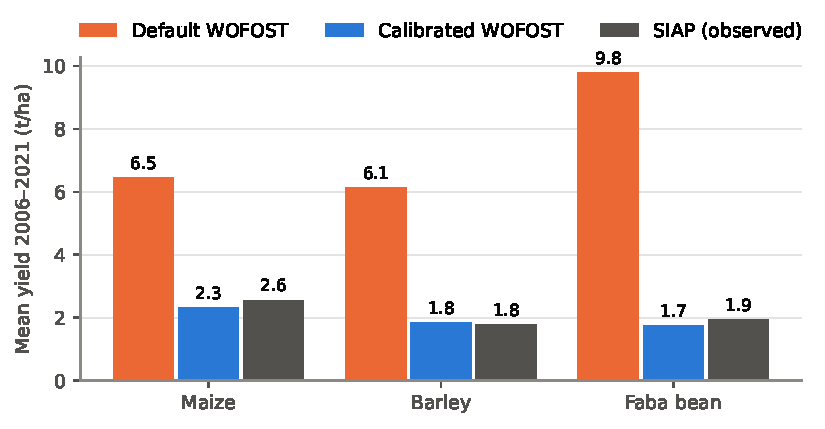
\includegraphics[width=0.85\linewidth]{figures/calibration_levels.pdf}
\caption{Mean yield over the fit years: the calibrated model (blue) now sits next to SIAP (gray).}
\label{fig:levels}
\end{figure}

\paragraph{How to read the results.}
\begin{itemize}[leftmargin=*]
  \item \textbf{The level is fixed.} In the fit years the calibrated means are within 0.06 (barley), 0.20 (faba bean)
        and 0.25 (maize) t/ha of SIAP. The \code{farm_gap} correction factors over 2006--2025 go from 0.42, 0.28 and
        0.18 to 1.14, 0.98 and 1.01.
  \item \textbf{The calibrated model does not beat the SIAP average.} In the fit years, climatology has a lower RMSE
        than the calibrated model for every crop. In the holdout, the calibrated model only edges out climatology for
        barley and faba bean, and persistence beats both by far: those SIAP series barely change from one year to the
        next. For maize, the calibrated model is worse than climatology in both periods (skill \(-0.53\) and
        \(-0.29\)). With \(r = 0.11\), even the best possible rescaling \(a + b\,y^{\mathrm{sim}}\) fitted to the
        observations would reach a skill of only \(1 - \sqrt{1 - r^2} = 0.006\): getting the level right cannot make the
        model beat the average; the missing year-to-year pattern is what keeps it behind. In 2022--2025, 2023 alone
        makes up 95\% of the maize squared error.
  \item \textbf{Year-to-year agreement is poor.} Calibrated maize has \(r = 0.11\) in the fit years. Its swings are
        about as large as the observed ones (standard deviation 0.88 vs 0.72 t/ha) but fall in the wrong years
        (Figure~\ref{fig:years}): it reproduces the 2011 loss but also invents losses in 2010, 2012 and 2020 and misses
        the 2019 loss. Faba bean is too steady (0.23 vs 0.51 t/ha) and does not follow SIAP's decline from 2.6 t/ha
        in 2005--2009 to about 1.2 in recent years, hence its holdout bias of +0.6 t/ha.
  \item \textbf{Maize sits on a steep slope.} Calibrated maize yields 2.0 t/ha at photosynthesis \(\times 0.45\) and
        2.8 at \(\times 0.5\) (Figure~\ref{fig:maize}). Small changes in the year's conditions push it across that
        slope, which is part of why its year pattern is erratic.
  \item \textbf{2023.} Calibrated maize gives 2.0 t/ha in 2023 in every rotation, against SIAP's 4.0.
\end{itemize}

\begin{figure}[H]
\centering
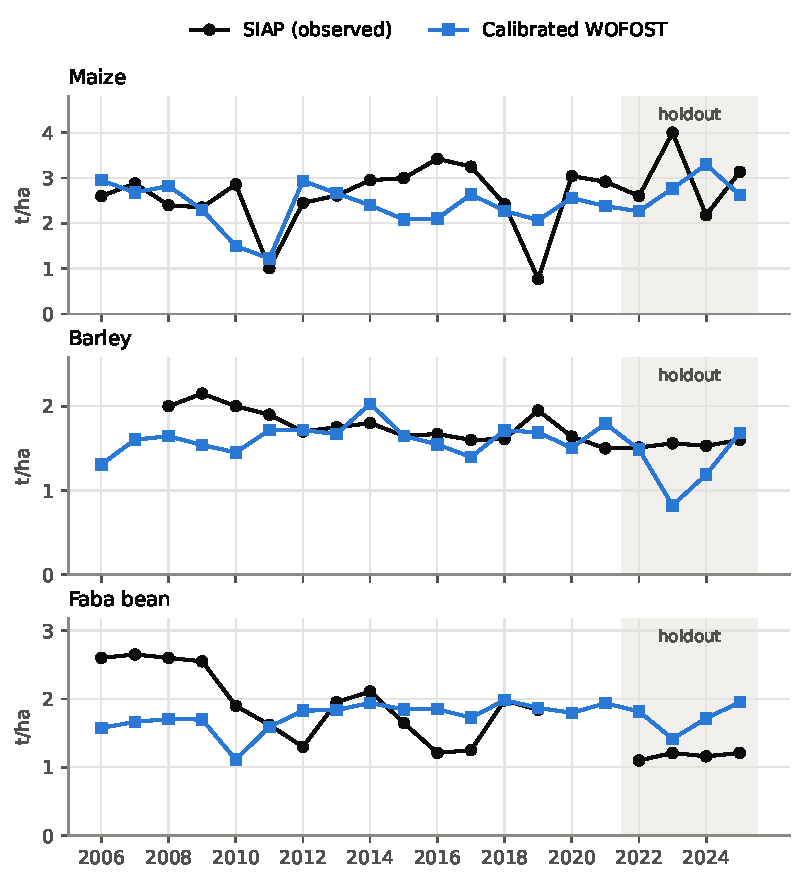
\includegraphics[width=0.88\linewidth]{figures/calibration_years.pdf}
\caption{Year by year: calibrated WOFOST (blue squares) against SIAP (black dots) and the climatology baseline
(dashed). The shaded years are the holdout. Missing black dots are years without SIAP data.}
\label{fig:years}
\end{figure}

\begin{figure}[H]
\centering
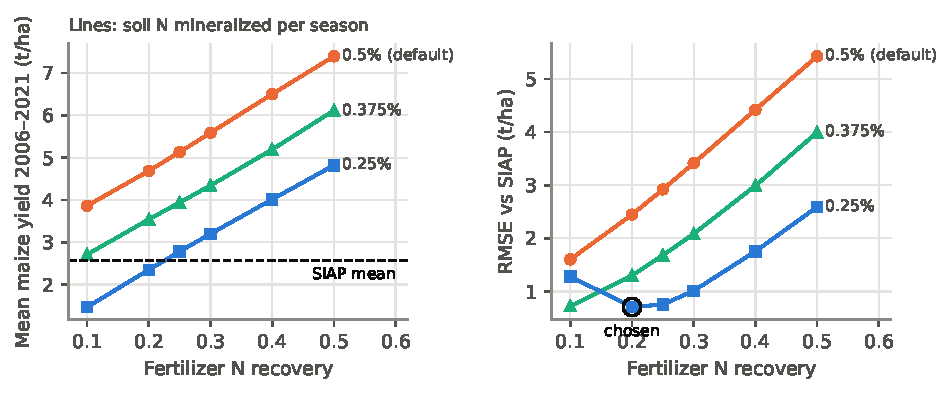
\includegraphics[width=\linewidth]{figures/calibration_maize_grid.pdf}
\caption{The maize step of the search at the chosen phenology (\(\times 0.8\)). Left: mean maize yield; the dashed line
is the SIAP mean. Right: yield without fertilizer divided by yield with fertilizer; the shaded band is the trial's
0.93 \(\pm\) 0.1. The circle is the chosen candidate. Only low photosynthesis reaches the farm level while keeping
the trial's small fertilizer response.}
\label{fig:maize}
\end{figure}

\begin{figure}[H]
\centering
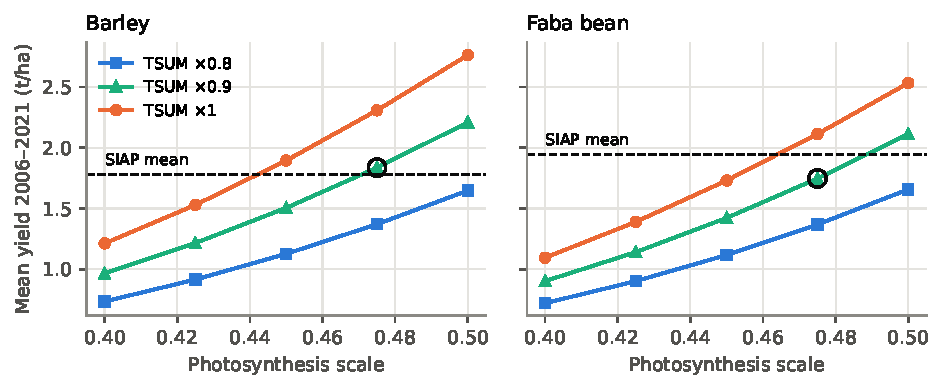
\includegraphics[width=\linewidth]{figures/calibration_photosynthesis.pdf}
\caption{The barley and faba bean steps (fertilizer N recovery 0.5). Each line is a phenology scale; the circled
point was chosen; the dashed line is the SIAP mean.}
\label{fig:photo}
\end{figure}

\section*{9. What this means for the rotation results}

The calibrated model reaches the farm level by lowering photosynthesis, not nitrogen, so nitrogen hardly limits
calibrated maize:
\begin{center}\small
\begin{tabular}{lrrrr}
\toprule
Mean yield, all years 2006--2021 (t/ha) & \multicolumn{2}{c}{Default model} & \multicolumn{2}{c}{Calibrated model} \\
 & with fertilizer & without & with fertilizer & without \\
\midrule
Maize & 6.47 & 1.92 & 2.31 & 2.30 \\
Barley & 6.15 & 3.90 & 1.81 & 1.81 \\
Faba bean & 9.81 & 9.77 & 1.77 & 1.77 \\
\bottomrule
\end{tabular}
\end{center}
As a result, calibrated maize after barley or after faba bean (2.32 t/ha) yields the same as maize after maize
(2.31 t/ha). The rotation benefits reported with the default model (EXPLORATION.md) need a second look too:
\begin{itemize}[nosep]
  \item In the baseline, maize--faba bean gave +0.63 t/ha over maize every year (2006--2025). That advantage comes
        entirely from the 2023 continuous-maize failure of Section~5 (+12.7 t/ha that year); without 2023 it is
        \(-0.003\) t/ha.
  \item With 20\% less rain and half fertilizer, the +1.0 t/ha advantage is real in the default model (+0.94 over
        2006--2021) and comes through nitrogen left by the faba bean. In the calibrated model nitrogen hardly limits
        maize, so that benefit would likely shrink (not simulated here).
\end{itemize}
If the Texcoco trial is right that nitrogen barely limits maize there, the simulated rotation benefits are
overstated. If farms are in fact more nitrogen-limited than the station, the first calibration was closer. SIAP cannot
tell which, so this needs field data on both fertilizer response and rotations.

\section*{10. Limits you should know about}

\paragraph{1. One station trial decides the nitrogen split.} Without the trial constraint, the best maize candidate
cut nitrogen instead (RMSE 0.87), with a no-fertilizer ratio of 0.26. With it, any low-photosynthesis candidate passes,
because farm-level maize needs little nitrogen (Section~6). The trial itself is matched only with more soil N than the
default (95--100 vs 64 kg per season), and the station's soil is likely more fertile than the average farm field. The
model's no-fertilizer runs are also 16 straight seasons without fertilizer, harsher than a one- or two-season trial.

\paragraph{2. Photosynthesis absorbs everything WOFOST does not simulate.} Weeds, pests, diseases, plant density and
local varieties are all lumped into one number per crop. It gets the level right, but it is not a measurement of any
of them.

\paragraph{3. Phenology is not pinned by observations.} We have no observed flowering or maturity dates, so
phenology was bounded by agronomic judgment rather than fitted to dates. Maize chose the shortest allowed cycle, and
several choices are near ties: faba bean's best three candidates have RMSE 0.606, 0.607 and 0.612, so its phenology is
barely identified.

\paragraph{4. The observations are coarse.} SIAP numbers are municipal estimates, often rounded (2.6, 2.4), and
recent barley and faba bean figures describe 4--12 hectares (31 and 18~ha of barley in 2017 and 2018). Faba bean's
decline over time is not explained by weather.

\paragraph{5. One point represents the whole municipality.} One POWER grid cell and one soil point; real fields
differ in soil depth (e.g.\ \emph{tepetate} layers), sowing date and management. The model's weather is also about
2.5\,\(^\circ\)C colder than the fields (Section~5).

\paragraph{6. Reproducibility.} PCSE re-downloads NASA POWER weather when its cache is older than 90 days, so the
saved runs (weather cached on 2026-10-12) cannot be reproduced exactly after about 2027-01-10. \code{calibration.json}
records the weather date, git commit and PCSE version, and \code{requirements.txt} pins PCSE 6.0.13 because
\code{wofost_rotations.py} patches that version.

\section*{11. How to use it and reproduce it}

Everything is opt-in; nothing changes for existing commands. From the repository root:
{\small
\begin{verbatim}
# One-at-a-time diagnostics, Table 2 (about 2 min, fit years only)
python -m src.crop_models.calibration --sensitivity
# The fertilizer-trial check of Section 6 (about 1 min)
python -m src.crop_models.calibration --station-check
# The search (about 13 min on 8 cores); writes fit_history.csv and fitted_knobs.json
python -m src.crop_models.calibration --fit
# Calibrated baseline -> data/rotations_calibrated/ (other scenarios with --scenarios)
python -m src.crop_models.calibration --simulate
python -m src.crop_models.calibration --simulate --scenarios baseline rain80
# The figures of this document
python docs/technical_report/make_calibration_figures.py
# Unit tests, including tests/test_calibration.py
python -m unittest discover -s tests
\end{verbatim}}
\sloppy
Files produced in \code{data/rotations_calibrated/}:
\begin{itemize}[nosep]
  \item \code{baseline.csv} (and any other scenario requested): the same columns as the default runs, with the
        scenario named \code{baseline_calibrated}, so default and calibrated runs can be loaded together;
  \item \code{calibration.json}: the knobs, fit and holdout years, versions, weather date and the scores of
        Table~\ref{tab:results};
  \item \code{fit_history.csv} and \code{fitted_knobs.json}: every candidate tried in the search and the chosen knobs
        (copy them into \code{CALIBRATED} after a refit);
  \item \code{sensitivity.csv} and \code{station_check.csv}: Table~\ref{tab:sens} and the trial check of Section~6.
\end{itemize}
The farmer notebook still loads the default runs and rescales them with \code{farm_gap} factors. This compares the
calibrated run with SIAP instead:
{\small
\begin{verbatim}
calibrated = load_seasons(["data/rotations_calibrated/baseline.csv"])
farm_gap(calibrated, siap, scenario="baseline_calibrated")
\end{verbatim}}

\section*{12. Glossary}

\begin{description}[leftmargin=0pt, itemsep=2pt, font=\normalfont\bfseries]
  \item[Area weighting] Combining simulated maize so that each previous crop counts by the share of maize fields
        that followed it, from SIAP areas.
  \item[Calibration] Adjusting a few model parameters so the model's output matches local observations.
  \item[Candidate] One combination of knob values tried by the search.
  \item[Climatology] A naive prediction: the average observed yield of the fit years, every year.
  \item[Coordinate search] Fitting one group of knobs (here, one crop) at a time while keeping the others fixed.
  \item[Correlation \(r\)] Whether simulated and observed good and bad years line up; ignores the level.
  \item[Grid search] Trying every combination of a short list of values for each knob.
  \item[Holdout] Years kept out of the search and used only to test the result.
  \item[Mineralization] Release of plant-available nitrogen from soil organic matter by microbes.
  \item[N recovery] The share of applied fertilizer nitrogen that the crop can actually take up.
  \item[Overfitting] Matching the fit years' noise so closely that new years are predicted badly.
  \item[Persistence] A naive prediction: last year's observed yield.
  \item[Phase] Where in its sequence a rotation starts; every phase is simulated so every crop appears each year.
  \item[Phenology] The timing of crop development (emergence, flowering, maturity).
  \item[RMSE] Root mean square error: the typical size of the difference between simulation and observation, in t/ha.
  \item[SIAP] Mexico's agri-food and fisheries information service, source of the observed yields.
  \item[Skill score] \(1 - \RMSE/\RMSE_{\text{climatology}}\): above 0 beats the average, below 0 does worse.
  \item[Spin-up] The first simulated year, discarded because it starts from assumed soil conditions.
  \item[TSUM] Thermal time (degree-days) a crop needs to reach flowering (TSUM1) or maturity (TSUM2).
  \item[Yield per sown hectare] Production divided by the area sown, so lost fields count as zero yield.
\end{description}

\end{document}
